
%!TEX root = CooperBarba2014.tex

\subsection{Discretization}

 \begin{figure}[b]
   \centering
   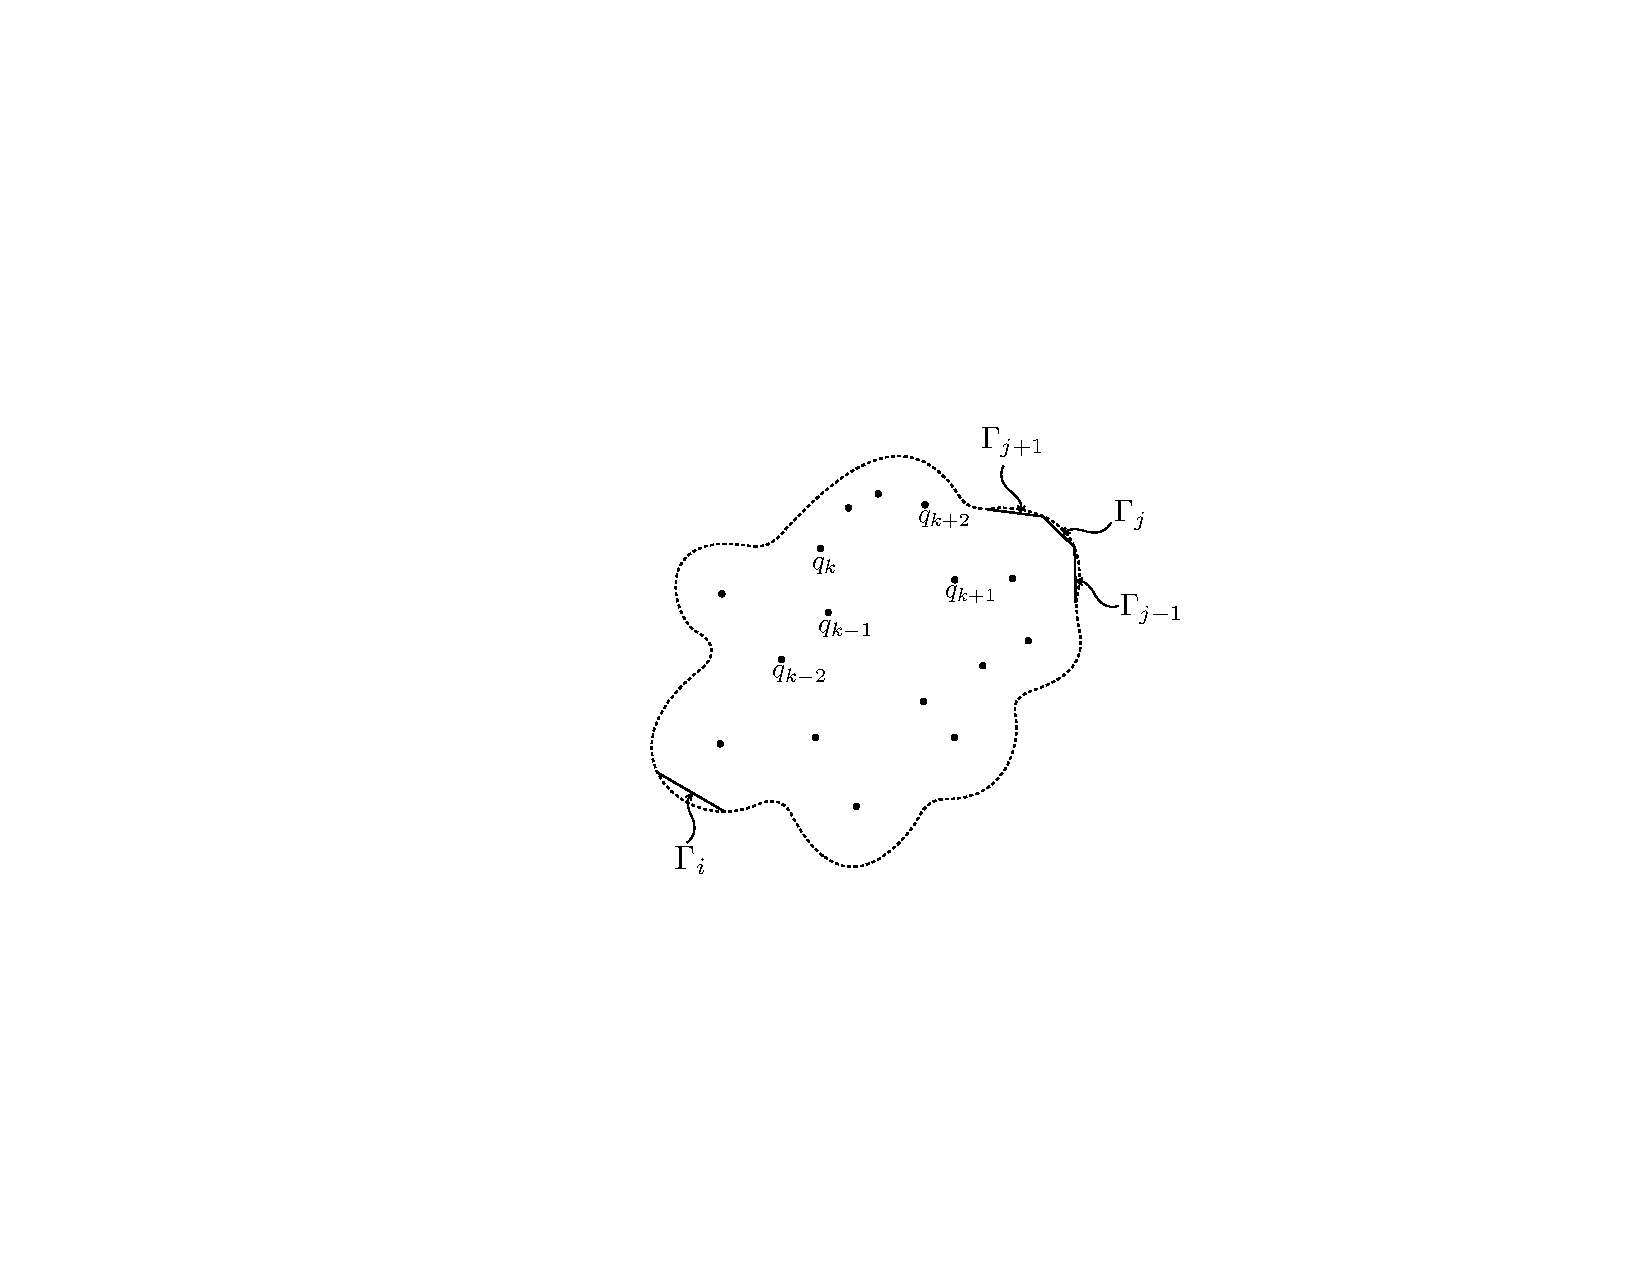
\includegraphics[width=0.4\textwidth]{Figure3.pdf} 
   \caption{Discretization of a molecular surface. $\Gamma_i$ is the panel where the collocation point resides and $\Gamma_j$ the panel being integrated.}
   \label{fig:molecule_disc}
\end{figure}

To numerically solve the system in \eqref{eq:integral_eq}, we discretize the boundaries into flat triangular panels and assume that $\phi$ and $\frac{\partial \phi}{\partial \mathbf{n}}$ are constant within those panels. Then, we collocate the discretized equation on the center of each panel to transform the integral operators in the matrix equation \eqref{eq:matrix_dphi} into block matrices of size $N_p \times N_p$, where $N_p$ is the number of panels. Each entry of the block matrix is an integral over one panel ($\Gamma_j$), evaluated on the center of panel $\Gamma_i$:
%
\begin{align} \label{eq:layers_element}
K_{L,ij} &= \int_{\Gamma_j} \frac{\partial}{\partial \mathbf{n}} \left[ G_L(\mathbf{r}_{\Gamma_i},\mathbf{r}_{\Gamma_j}) \right]\mathrm{d} \Gamma_j, \nonumber \\
V_{L,ij} &= \int_{\Gamma_j} G_L(\mathbf{r}_{\Gamma_i},\mathbf{r}_{\Gamma_j})  \mathrm{d} \Gamma_j.
\end{align}

In our numerical solution, integrals are calculated in three ways, depending on how close the panel is to the collocation point. When the collocation point is inside the element being integrated, we use a semi-analytical technique, \cite{ZhuHuangSongWhite2001} with Gauss points placed along the edges of the element. If the integrated element is closer than $2L$ from the collocation point ---where $L = \sqrt{2\cdot \text{Area}}$--- we use a fine Gauss quadrature rule, with 19 or more points per element. Beyond a distance of $2L$, elements have only 1, 3, 4 or 7 Gauss points, depending on the case.

We solve the resulting linear system with a general minimal residual method (\gmres). We accelerate the matrix-vector product in each iteration of the \gmres using a treecode algorithm, making the computer time scale as $O(N\log N)$, rather than the naive $O(N^2)$. More details on our implementation of the \bem can be found in our earlier work,\cite{CooperBarba-share154331} and a companion paper.\cite{CooperBarba2015a}
